\documentclass[12pt, oneside]{article}
\usepackage[letterpaper, margin=1in]{geometry}
\usepackage[english]{babel}
\usepackage[utf8]{inputenc}
\usepackage{amsmath}
\usepackage{amsfonts}
\usepackage{amssymb}
\usepackage{tikz}
%\usepackage{tkz-fct}

\usepackage{fancyhdr}
\pagestyle{fancy}
\fancyhf{}
\rhead{\thepage \\Name: \hspace{1.5in}.\\}
\lhead{BECA / Dr. Huson / 11.1 IB Math SL \\* 29 May 2018 \\* \textbf{Do Now Quiz: Using the unit circle and the law of sines}}

\vspace{1cm}

\renewcommand{\headrulewidth}{0pt}

\title{Problem set template}
\author{Chris Huson}
\date{May 2018}

\begin{document}
%\maketitle

\subsubsection*{\\* \textnormal{Closed book \& no notes. Show work in space provided. Work problems in order.}}

\begin{enumerate}

\item Given a circle with radius of one, centered on the origin. An angle with measure $30^\circ$ is placed in standard position. Mark the point $A$, the intersection of the circle and angle ray, as an ordered pair.
\begin{center}
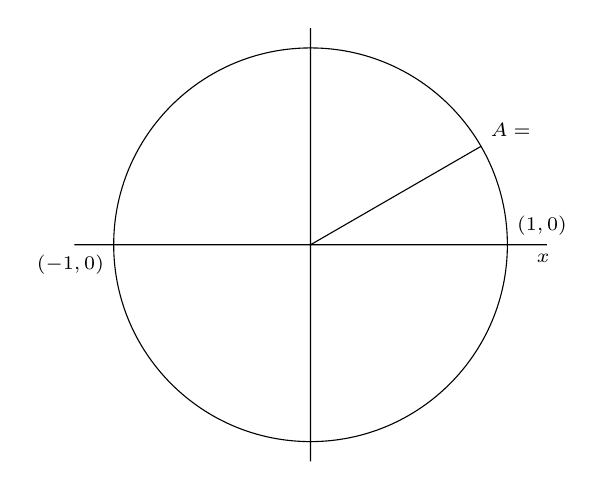
\begin{tikzpicture}[scale=2.5]
  \draw[font=\scriptsize]
    (-1.2, 0) -- (1.2, 0)
    (0, -1.1) -- (0, 1.1)
    (0, 0) -- (0.866, .5) node[above right] {$A=$}
    (0, 0) circle[radius=1]
    (-1, 0) node[below left] {$(-1,0)$}
    (1, 0) node[above right] {$(1,0)$}
    (1.1, 0) node[below right] {$x$}
    ;
\end{tikzpicture}
\end{center}
\begin{enumerate}
      \item Write down the value of $\sin{30^\circ}$\\[0.25in]
      \item  Write down the value of $\cos{30^\circ}$\\[0.25in]
\end{enumerate}


\item Triangle $ABC$ has $\hat{A}=40^\circ$, $AB=7 \text{ cm}$, \& $BC=6 \text{ cm}$. Find the measure of $\hat{C}$:
\begin{enumerate}
      \item Write down the law of sines, substituting appropriate values.\\[0.5in]
      \item Solve for the measure of angle $C$
\end{enumerate}
\begin{center}
\begin{tikzpicture}[scale=0.6]
\draw (0,0) node[anchor=north]{$A$}
  -- (12,0) node[anchor=north]{$C$}
  -- (6.75,6) node[anchor=south]{$B$}
  -- cycle;
  %(0,3) node[anchor=south]{$40^\circ$};
  %\draw [dashed] (1.5,0) -- (1.5,4.2);
\end{tikzpicture}
\end{center}


\newpage
\subsubsection*{Early finishers}

\item The polynomial $f(x)=x^3-13x-12$ is shown on the graph below. What is the slope between the local minimum at $x=2$ and the $x$-intercept at $x=4$? This is called the \emph{average rate of change} between $x=2,4$.
\begin{center}
    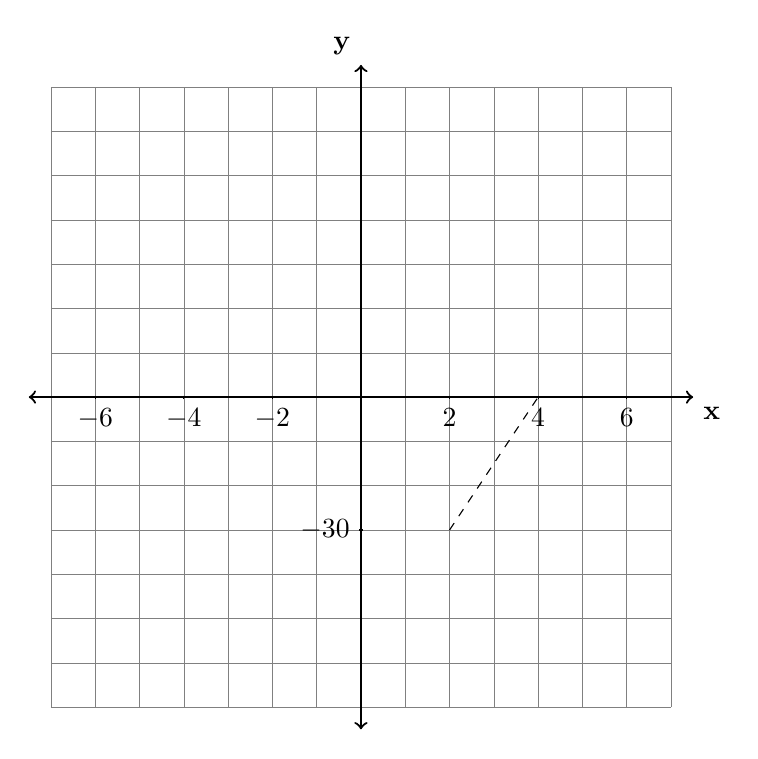
\begin{tikzpicture}[scale=2.25/4]
    \draw[step=1cm,gray,very thin] (-7,-7) grid (7,7);
    \draw[thick,<->] (-7.5,0) -- (7.5,0) node[anchor=north west] {\textbf{x}};
    \draw[thick,<->] (0,-7.5) -- (0,7.5) node[anchor=south east] {\textbf{y}};
    \foreach \x in {-6, -4, -2, 2, 4, 6} \draw (\x cm,1pt) -- (\x cm,-1pt) node[anchor=north] {$\x$};
    \foreach \y in {-3} \draw (1pt,\y cm) -- (-1pt,\y cm) node[anchor=east] {$-30$}; %{$\y$};
%    \tkzInit[xmin=-6,xmax=5,ymin=-7,ymax=7,ystep=1]   
%    \tkzFct[color=black,thick,<->,domain = -4.3:4.9] {0.1*(x+3)*(x+1)*(x-4)};
    \draw [dashed] (2,-3) -- (4,0);
    \end{tikzpicture}\\*[1.5in]
\end{center}

\item Simplify the expression $\displaystyle 32^{\frac{1}{5}}$. Explain your result.

\end{enumerate}
\end{document}
